\documentclass[twocolumn]{article}
\usepackage{fancyhdr}
\usepackage{pgf}
\usepackage{multicol}
\usepackage{amsmath}
\usepackage{enumerate}
\usepackage{listings}
\usepackage[top=2in, bottom=1.5in, left=1in, right=1in]{geometry}
\usepackage{graphicx}
\usepackage{tabularx} 

\lstset{
	tabsize=4,
        basicstyle=\scriptsize,
        %upquote=true,
        aboveskip={1.5\baselineskip},
        columns=fixed,
        showstringspaces=false,
        breaklines=true,
        prebreak = \raisebox{0ex}[0ex][0ex]{\ensuremath{\hookleftarrow}},
	frame=none,
        showtabs=false,
        showspaces=false,
        showstringspaces=false,
        identifierstyle=\ttfamily,
        keywordstyle=\color[rgb]{0,0,1},
        commentstyle=\color[rgb]{0.133,0.545,0.133},
        stringstyle=\color[rgb]{0.627,0.126,0.941},
	language=C++
}

\def\SUBJECT{ECE 486}
\def\TOPIC{Project 2 \\ Branch and Branch Target Prediction}
\def\AUTHOR{Vernon \textsc{Jones} \\ Tyler \textsc{Tricker}}
\def\INSTRUCTOR{Mark \textsc{Faust}}

%*******************Page layout
\pagestyle{fancy}
\lhead{\AUTHOR}
\chead{\SUBJECT: \TOPIC}
\rhead{\thepage}
\fancyfoot{}


\begin{document}
\begin{titlepage}
 \begin{center}
 \newcommand{\HRule}{\rule{\linewidth}{0.5mm}}
% Upper part of the page. The '~' is needed because \\
% only works if a paragraph has started.

\textsc{\LARGE Portland State University}\\[1.5cm]

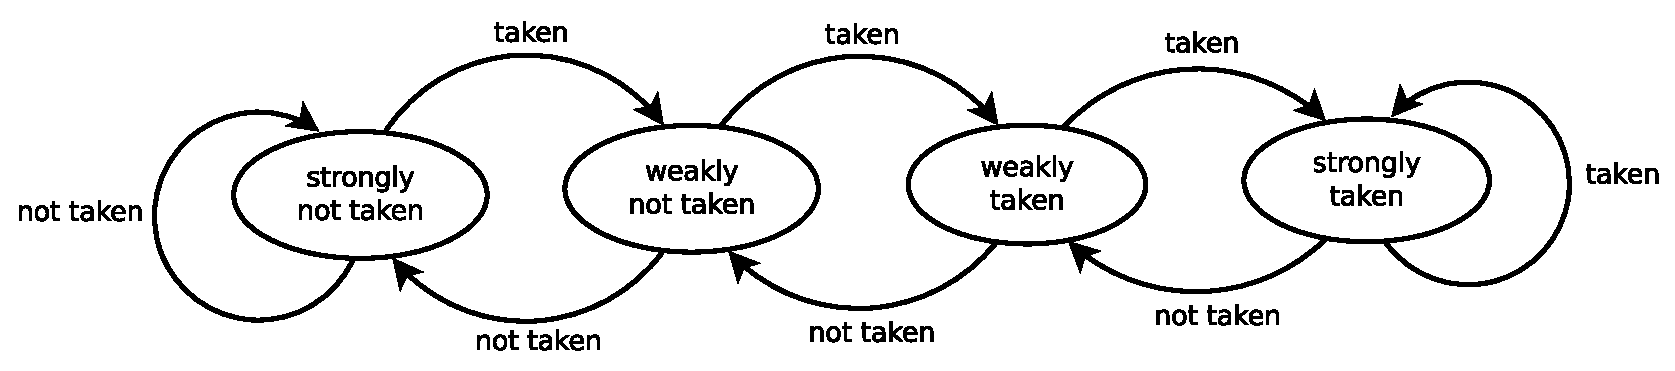
\includegraphics[width=0.5\textwidth]{./logo}~\\[1cm]

\textsc{\Large \SUBJECT}\\[0.5cm]

% Title
\HRule \\[0.4cm]
{ \huge \bfseries \TOPIC}\\[0.4cm]

\HRule \\[1.5cm]

% Author and supervisor
\begin{minipage}{0.4\textwidth}
\begin{flushleft} \large
\emph{Author:}\\
\AUTHOR
\end{flushleft}
\end{minipage}
\begin{minipage}{0.4\textwidth}
\begin{flushright} \large
\emph{Instructor:} \\
\INSTRUCTOR
\end{flushright}
\end{minipage}

\vfill

% Bottom of the page
{\large \today}

\end{center}

\end{titlepage}

\section{Introduction}
This project simulates the Branch Predictor from the Alpha 21264 and implements a branch target predictor of our own design.

\subsection{Branch Target Prediction}
The Alpha 21264 Microprocessor predicted branch outcomes using a global predictor, and a local predictor. A tournament predictor would then choose which predictor to use based on path history.

\subsection{Branch Target Buffer}
The Branch Target Buffer uses a PC-relative and a PC-absolute cache. Targets that are close to the current instruction are placed into the PC-relative cache. A circular return stack is used for returns. All caches are exclusive.


\section{Methods of Analysis}
\subsection{Trace File Analysis}
The main strategy applied in the design of this project was divide and conquer; In order to keep the code as independent as possible the different types of instructions were decoupled. After doing a quick statistical analysis of the break down of instruction types conditionals, calls and returns are the most frequently encountered, in that order. Conditional branches comprised a significant majority of all branches encountered in any of the traces and had a very interesting pattern to them.
\begin{figure}
\begin{center}
\includegraphics[width=7.4cm]{"./Conditional Branches DIST-INT-4-histogram"}
\caption{Graph showing the typical relative offset breakdown of conditional branches, y axis is in frequency}
\end{center}
\end{figure}
\subsection{Trace Analysis}
By analyzing the relative branching distances of branch instructions an interesting pattern emerged in Conditional Branches. A majority of them are backward branching and nearly all of them are contained within 1024 bytes. This information greatly influenced our design decisions outlined in the next major section.
\begin{figure}
\begin{center} 
\includegraphics[width=7.4cm]{"./Calls Branches DIST-SERV-4-density"}
\includegraphics[width=7.4cm]{"./Calls Branches DIST-SERV-4-histogram"}
\caption{Graphs showing the complications in predicting functional calls efficiently}
\end{center}
\end{figure}
Functional calls were more staggered as far as PC relative. Across all of the traces however there were interesting density patterns for calls. Almost all of the branches are concentrated in two areas. Which directly corresponds to a typical virtual address space implemented on most operating systems. The density graph shows a typical $.text$ segment and a shared library address space. With branches rare or non existent in the stack and heap. The exception to this is some of the server trace files, which is quite possibly an application level virtual machine looking at how many times it calls into an area normally reserved to the heap.

\subsection{Memory Analysis}
8KB was the non-negotiable limit required for the project. To get an overview of the budget requirements and range of space that can be covered a spreadsheet was made showing a variety of cache configurations. A copy of this is in the bit Budget Appendix. This was done in a standard spreadsheet for quick turn around.


\section{Design}
The Branch Target Buffer does a target lookup on all branch types. The Alpha Predictor only returns a prediction on a conditional branch.

\subsection{Alpha Predictor Design}
The Alpha Predictor uses global prediction, and local prediction. The global prediction is indexed by a global path history into an array of saturating counters. The local prediction is indexed by PC into a local history table; the result of the local history table is then used to index into an array of saturating counters.

\subsection{Return Address Stack Design}
The Return Address stack is implemented as a dirty circular buffer. The stack is dirty because if the stack runs out of entries it will loop around and continue to return old values in the stack. When addresses are pushed onto stack they have to potential to overwrite old values on the bottom of the stack. This is useful in the rare cases that there is a recursive function that is not tail call optimized as the stack will continue to return roughly the same sequence as was pushed on to it. When a call function is encountered the address of the next instruction gets pushed onto the stack. When a return instruction is encountered an address gets popped from the stack and predicted.

\subsection{Branch Target Buffer Design}
The Branch Target Buffer consists of an absolute cache, a PC-relative cache, and a circular return stack. On a prediction both caches are queried and either cache that makes a prediction is the value of the prediction. Values are stored in these caches depending on whether the difference between the branch instruction and branch target differ by less than 1024 bytes. If it can be represented than the prediction target gets put into the PC-relative cache, otherwise it goes into the absolute cache. 

\subsection{Relative vs Absolute}
Two caches are utilized for the Branch Target Buffer. A larger PC-relative cache is used for targets that are less than 1024 absolute bytes away from the instruction. This means that only 11 bits are needed for the data section of the PC-relative cache. This, combined with a 25-bit tag size, a four-way cache and 4 bits of LRU overhead per set, gives a total set size of 148 bits. 148 bits per set, with 128 set, gives a cache size of 18,944 bits, or 18.5Kbits.

The absolute cache directly uses the lower-order 6 bits of the address to index into a table. It has a data size of 32-bits with a 26-bit tag size. With a four-way cache and 4 bits of LRU overhead per line, the total line size is 236 bits per line. 236 bits per set, with 64 set, gives a cache size of 15104 bits, or 14.75Kbits.

This means that the relative and absolute caches use 34048 bits, or 33.25Kbits. 


\section{Testing Methodology}
We tested stuff and junk

\subsection{Relative vs Absolute}


\onecolumn
\section{Results}
Predictor results from trace files
\lstinputlisting{../src/results.log}

\section{Appendix Code - predictor.h}
\lstinputlisting[language=C++]{../src/predictor.h}
\section{Appendix Code - predictor.cc}
\lstinputlisting[language=C++]{../src/predictor.cc}
\end{document}
